%% ****** Start of file apstemplate.tex ****** %
%%
%%
%%   This file is part of the APS files in the REVTeX 4 distribution.
%%   Version 4.1r of REVTeX, August 2010
%%
%%
%%   Copyright (c) 2001, 2009, 2010 The American Physical Society.
%%
%%   See the REVTeX 4 README file for restrictions and more information.
%%
%
% This is a template for producing manuscripts for use with REVTEX 4.0
% Copy this file to another name and then work on that file.
% That way, you always have this original template file to use.
%
% Group addresses by affiliation; use superscriptaddress for long
% author lists, or if there are many overlapping affiliations.
% For Phys. Rev. appearance, change preprint to twocolumn.
% Choose pra, prb, prc, prd, pre, prl, prstab, prstper, or rmp for journal
%  Add 'draft' option to mark overfull boxes with black boxes
%  Add 'showpacs' option to make PACS codes appear
%  Add 'showkeys' option to make keywords appear
%\documentclass[aps,prb,preprint,superscriptaddress,showkeys,endfloats]{revtex4-1}
%\documentclass[aps,prb,preprint,superscriptaddress,showkeys]{revtex4-1}
\documentclass[aps,prl,reprint,superscriptaddress,showkeys]{revtex4-1}
\usepackage{amsmath}
\usepackage{color}
\usepackage{graphicx}
\usepackage{dcolumn}
\usepackage{verbatim}
\usepackage{epstopdf}
\usepackage{inputenc}
\newcolumntype{d}{D{.}{.}{-1}}





\begin{document}




%\title{Fully parallel methods for calculation of partition functions for systems with known number of states with application to crystalline Li$_2$OHCl and Li$_2$OHBr}
\title{First principles calculation of configurational energy density of states in LLTO with new Wang and Landau algorithm variant }

\author{Jason D. Howard}
\affiliation{Materials Science Division, Argonne National Lab, Lemont, IL, 60439, USA}

\date{\today}

%\begin{abstract}
%\input{abstract}
%\end{abstract}


\begin{acknowledgments}
\end{acknowledgments}
\begin{abstract}
In this work  a variant of the Wang and Landau algorithm   for calculation of  the configurational energy density of states is proposed. The algorithm is referred to as B$_L$ENDER, which is an acronym for B$_L$end Each New Density Each Round and an  adjective for  how it was created and functions. The algorithm was developed for the purpose of working towards the goal of using first principles simulations, such as density functional theory, to calculate the partition function of disordered sub lattices in crystal materials. The expensive calculations of first principles methods make a parellel aglorithm necessary for a practical compuation of the configurational energy density of states within a supercell approximation of a solid state material. The developed algorithm is natural to paralleize and is developed from a self consistent perspective.  The algorithm develped in this work is tested with the 2d Ising model to bench mark the algorithm and to help provide insight for implementing the algorithm to a materials science application. The algorithm is then applied to the lithium and lanthunum sublattice of the solid state lihithium ion conductor Li$_{0.5}$La$_{0.5}$TiO$_{3}$. This was done to help understand the disordered nature of the lithium and lanthanum. The results find overall that the algorithm performs very well for the 2-d Ising model and that the results for Li$_{0.5}$La$_{0.5}$TiO$_{3}$ are consistent with experiment while providing additional insight into the lithium and lanthunum ordering in the material. 
\end{abstract}
\maketitle
\section{Introduction}
For crystalline  materials  with disordered sub-lattices such as the Li-ion solid state electrolyte LLTO it is desirable to calculate from first principles methods(such as density functional theory\cite{kohn:1965}) the configurational  energy density states $G(E_j)$. Here the energy density of states is meant to correspond to the energies of the distinct lattice configurations. With the energy density of states the partition function,
\begin{equation}
\begin{split}
Z = \sum_{i}^{\Omega}e^{\frac{-e_i}{k_B T} }= \sum_{j}^{\Pi}G(E_j)e^{\frac{-E_j}{k_BT}} \;,
\end{split}
\label{partition}
\end{equation}
can be  determined and from it many important thermodynamics properties such as the free energy, entropy, specific heat, and ensemble averages calculated. In Eq. (\ref{partition}), $\Omega$ corresponds to the number of possible configurations and energies in the set $\{\Sigma_i,e_i\}_\Omega$, $\Pi$ to number of possible distinct energies $E_j$, $k_B$ is Boltzman's constant, and $T$ is the temperature. One method to solve this problem could be temperature dependent simulations involving the  Metropolis algorithm and histogram re-weighting techniques\cite{metropolis_equation_1953, landau_MC_simulations}.   Another algorithm called the  Wang and Landau algorithm\cite{WL_phys_rev_lett} has been developed which is temperature independent and is based on a random walk in energy space.  An issue with these algorithms in use with first principles methods such as density functional theory is the large number of iterations needed which would require a prohibitively long wall time at the current performance power of computers.  In this paper a method is proposed that combines the use of random sets along with the importance sampling method of the Wang and Landau algorithm that is meant to work towards the goal of highly parallel importance sampling algorithms that mesh well with high performance computing architectures and have a minimum of parmaters for implementation. The algorithm developed in this work is referred to as the B$_{L}$ENDER (B$_{L}$end Each New Density Each Round) algorithm. 
    The Wang and Landau method does have parallel versions, including  restricting random walkers to specific energy ranges or allowing the walkers to explore the entire space while periodically communicating with each other \cite{MP_Wang_Landau,P_imp_Wang_Landau, Hframe_Wang_Landau}.  In principle the different forms of the Wang and Landau sampling currently used are based around the concept of sampling until a flat historgram of the visted energies is reached followed by a reduction in the modification factor of the density of states. There have been advancements made in understanding how to reduce the modification factor by Belardinelli et al. \cite{saturation}. The novel aspect of the B$_{L}$ENDER algrotihm is a continuous modification of the modification factor to the  density of states using the current sum of the density of states. The algorithm in this work was also formulated in a self consistent fashion and is believed to naturally evolve to a flat histogram of the visted energy levels.  The  algorithm is also natural to parallelize as it is based on a set of random walkers that each can explore the entire energy range. 

   In this work the formulated algorithm is benched marked with the 2d Ising model as a standard means of testing if valadity.  The tests allow for comparision to exact results and to previous benchmarks of other algorithms. The tests with the 2d Ising model also allow for insight in how to implement the algorithm to a materials science problem. In this work the main goal was to calculate the configurational energy density of states of the lithium ion conductor Li$_{0.5}$La$_{0.5}$TiO$_3$.  This material is part of a family of possible stoiciometries Li$_{3x}$La$_{2/3 -x}$TiO$_3$ of interest as solid state lithium ion conductors\cite{domainboundaries,P4mmmstrucuture,imaginary_phonons,GENG2009555,peculiarities,LLTOreview,Li_La_ordering_computational}. For all of the possible stoiciometries there is a tendency towards ordering of the lithium and lanthanum into lithium rich layers and lanthanum rich layers.  The primary calculation of this work is that of the temperature dependant order parameter related to the lanthanum rich layer in Li$_{0.5}$La$_{0.5}$TiO$_3$. This calculation both serves to benchmark the application of the algorithm to a materials science problem with experimental knowns and to provide further insight into the physics of the material. 
   
   The rest of the article is organized as follows;  section explaining and motivating the new algorithm, a section bench marking the algorithm with the 2d ising model, then a section applying the algorithm to the Li$_{0.5}$La$_{0.5}$TiO$_3$ system followed by the conclusions. 

\section{Algorithm}
   
The B$_{L}$ENDER algorithm proposed in this work  is given as follows. It is noted that the following algorithm is in terms of producing a relative density of states $G_{r}(E_j)^I$, where $I$ is the iteration number. 

\begin{equation}
\begin{split}
&1.\hspace{0.125cm} G_{r}(E_j)^I ,\hspace{0.15cm}  \{\Sigma_{s},e_s\}_{\mathcal{S}}^I\\
&2. \hspace{0.125cm}\{\Sigma_{s},e_s\}_{\mathcal{S}}^I \rightarrow  \{\Sigma_{s}^{'},e_s^{'}\}_{\mathcal{S}}^I\\
&3. \hspace{0.125cm} \Sigma_{s}^{'I}, e_s^{'I} \rightarrow \Sigma_{s}^{I+1},e_s^{I+1}   \hspace{0.125cm} P = \hspace{0.075cm} min [1, G_r(e_s)^{I}/G_r(e_s^{'})^{I}]\\
& \hspace{0.125cm}else  \hspace{0.15cm} \Sigma_{s}^I, e_s^I \rightarrow \Sigma_{s}^{I+1}, e_s^{I+1}\\
&4. \hspace{0.125cm} G_{r}(E_j)^{I+1} =  \\
& G_{r}(E_j)^{I} + \frac{C_o \mathcal{H}(E_j,\{e_s\}_{\mathcal{S}}^{I+1}) }{ [\sum_j G_{r}(E_j)^{I}]^{\frac{1}{N} } }G_{r}(E_j)^{I} = \\
& G_{r}(E_j)^{I}( 1 +  \frac{C_o \mathcal{H}(E_j,\{e_s\}_{\mathcal{S}}^{I+1}) }{ [\sum_j G_{r}(E_j)^{I}]^{\frac{1}{N} } } )\\
\end{split}
\label{blender}
\end{equation}
Where  $G_{r}(E_j)^0 \equiv [1 +  \frac{C_o}{S}\mathcal{H}(E_j,\{e_s\}_{\mathcal{S}}^0)]$ with $\mathcal{H}(E_j,\{e_s\}_{\mathcal{S}})$ being a histogram function that counts the number of energies $E_j$ in the set $\{e_s\}_{\mathcal{S}}$. In this work $\{\Sigma_{s},e_s\}_{\mathcal{S}}^0$  is a randomly(uniformly) drawn set from the configuration space $\{ \Sigma_i, e_i \}_\Omega $. In the second step  a random change is applied to each element of the sampled set $\{\Sigma_{s},e_s\}_{\mathcal{S}}^I$ to produced a ``perturbed" set $ \{\Sigma_{s}^{'},e_s^{'}\}_{\mathcal{S}}^I$ , for the Ising model this could be randomly flipping a spin.  In the third step a random number is drawn between zero and one for every sampled configuration, if this number is less then the ratio of the current density of states $G_{r}(e_s)^{I}/G_{r}(e_s^{'})^{I}$ then the perturbed configuration and energy  $\Sigma_{s}^{'I},e_s^{'I}$  goes to $\Sigma_{s}^{I+1},e_s^{I+1}$,  else the unperturbed configuration and energy $\Sigma_{s}^{I},e_s^I$  goes to $\Sigma_{s}^{I+1},e_s^{I+1}$. This step (third) is dervied from the Wang and Landau method of sampling with probablity proportional to the inverse of the density of states.  In the fourth step a histogram of the updated $\{ e_s \}^{I+1}_{\mathcal{S}}$ energies is made and added (blended) into the current density of states $G_{r}(E_j)^I$   by multiplying  by a constant $C_{o}$(which affects the convergence properties) and the relative probability of each energy $E_j$ in the  intermediary density of states $G_{r}(E_j)^{I}$. The fourth step is also shown in terms of multiplication which is discussed later. In this work it was found  $C_{o}=\Omega^{\frac{1}{N}}$ was computationally efficient. After the algorithm is deemed to be complete it is necessary to re-normalize the iterated relative density of states $G_{r}(E_j)^f$ at the final iteration $I=f$ as follows, 
\begin{equation}
\begin{split}
&1. \hspace{0.125cm} A = \sum_jG_{r}(E_j)^f\\
&2. \hspace{0.125cm} G(E_j)\approx G_{r}(E_j)^f \frac{\Omega}{A} \;,
\end{split}
\label{renormalize}
\end{equation}
to produce the properly normalized estimated value of $G(E_j)$. In principle the $G_{r}(E_j)$ can also be renormalized based on information of the number of configurations in a given bin, for example if the ground state is known to have a given degenerancy.  

An important discussion point of this algorithm (Eq \ref{blender}) is the update of the relative density of states(step four) being presented as addition and multiplication. In the addition form the self consistent nature of the update is clear, in the sense that the  density of states is updated by adding a  piece proportional to the counts in the histogram of the random set times the relative proportion of  that energy level in the current estimate of the density of states.  In the typical Wang and Landau sampling the update of the density of states is preformed by multiplication combined with a periodic reduction of the multiplication factor. In the multiplication form of step four of this algorithm (Eq \ref{blender}) it is seen that the dependence on one over the sum of the density of states serves to naturally reduce the multiplication factor as the simulation progresses. The multiplication form is also useful when $\Omega$ is large and the sum of the density of states is larger than a typical floating point number. In this case the log of the density of states can be stored and the update performed through addition of logs. Taking $G_{r}^M \equiv  max[G_{r}(E_j)]$ the log of $\sum_j G_r(E_j)^{I}$ can be written as, 
\begin{equation}
\begin{split}
&G_{r}^{LS} \equiv \log[\sum_j G_{r}(E_j)^{I}] = \log[G_{r}^M \frac{\sum_j G_{r}(E_j)^{I}}{G_{r}^M}]=\\
&\log[G_{r}^M] + \log[\sum_j e^{\ln[G_{r}(E_j)] - \ln[G_{r}^M]} ] \;.
\end{split}
\label{Hls}
\end{equation} 
With $G_r^{LS}$ from Eq \ref{Hls} the $\log$ update form of step four of the algorithm (Eq \ref{blender}) can be written as the following, 
\begin{equation}
\begin{split}
& \log[ G_{r}(E_j)^{I}( 1 +  \frac{C_o \mathcal{H}(E_j,\{e_s\}_{\mathcal{S}}^{I+1}) }{ [\sum_j G_{r}(E_j)^{I}]^{\frac{1}{N} } } ) ]=\\
& \log[ G_{r}(E_j)^{I} ] + \log[1 +   \mathcal{H}(E_j,\{e_s\}_{\mathcal{S}}^{I+1})e^{\ln[C_o]-\frac{1}{N}G_{r}^{LS}}] \;.
\end{split}
\end{equation}
In this form  the alogrithm can be implemented even when $\Omega$ is large. To implement the ratio of the density of states in step two of the algorithm, 
\begin{equation}
e^{\ln[G_{r}(e_s)^{I}] - \ln[G_{r}(e_s^{'})^{I}]} \;,
\end{equation}
can be used.

\subsection{Rationale for Algorithm}

The above algorithm can be rationalized by considering the adiabatic properties of a more general historgram $\mathcal{H}(E_j,\{e_s\}_{\mathcal{S}\times\mathcal{I}})$. Where  $\mathcal{H}(E_j,\{e_s\}_{\mathcal{S}\times\mathcal{I}})$ is a historgram generated with $\mathcal{S}$ walkers simulated to $\mathcal{I}$ iterations using Wang and Landau importance sampling with respect to  a fixed estimate of the density of states $G_r(E_j)$.  Considering that the sampled  energies are being generated with a probablility proportional to  the exact density of states $G(E_j)$ and accepted  with propablity inversely proportional to the relavtive(estimate) of the density of states $G_r(E_j)$, a historgram $\mathcal{H}(E_j,\{e_s\}_{\mathcal{S}\times\mathcal{I}})$ in equilibrium with $G(E_j)$ and $G_r(E_j)$ should follow the proportionality, 
\begin{equation}
\mathcal{H}(E_j,\{e_s\}_{\mathcal{S}\times\mathcal{I}}) \propto   \frac{G(E_j)/\Omega}{G_r(E_j)/A} \; .
\label{proportanality}
\end{equation}
Where $A$ is the sum over $G_r(E_j)$. Consider here that $\mathcal{H}(E_j,\{e_s\}_{\mathcal{S}\times\mathcal{I}})$ is generated with a fixed $G_r(E_j)$ for a certain number of iterations $\mathcal{I}$, then its sum is $\mathcal{I}\times S$.  So in normalizing the proportionality in Eq \ref{proportanality} to $\mathcal{I}\times S$ we get,
\begin{equation}
\mathcal{H}(E_j,\{e_s\}_{\mathcal{S}\times\mathcal{I}}) =  \mathcal{S I}\frac{G(E_j)}{G_r(E_j)}  (\sum_j^{\Pi}\frac{G(E_j)}{G_r(E_j)})^{-1} \;.
\label{dervied_GE_GEr_relationship}
\end{equation}
Solving for the exact density of states gives,
\begin{equation}
G(E_j) = \mathcal{H}(E_j,\{e_s\}_{\mathcal{S}\times\mathcal{I}}) G_r(E_j)  \Phi \;,
\label{GEfromhist}
\end{equation}
where,
\begin{equation}
  \Phi \equiv \sum_j^{\Pi}\frac{G(E_j)}{G_r(E_j)}\frac{1}{\mathcal{S I}} \;. 
 \end{equation}
  A similar result, that the exact density of states is encoded in the average historgram of visited energies taken from a dynamic($G_r(E_j)$ changes) Wang and Landau simulation, was found by Zhou et al. \cite{understand_improve}. It is important to note that Eq \ref{GEfromhist} assumes that $\mathcal{H}(E_j,\{e_s\}_{\mathcal{S}\times\mathcal{I}})$ is in equilibrium and simulated to an abritary level of precision with respect to $G(E_j)$ and $G_r(E_j)$. In general we may assume an approximately equals in Eq \ref{GEfromhist}.  From Eq \ref{GEfromhist} it is important to note that $\Phi$ is equivalent for all energy levels and does not affect relative probablities.  In this sense we can rewrite  Eq \ref{GEfromhist} as an equation for updating the relative density of states as follows, 
 \begin{equation}
 G_r(E_j)^{I+1} = \mathcal{H}(E_j,\{e_s\}_{\mathcal{S}\times\mathcal{I}}) G_r(E_j)^I  \phi \;.
 \label{Grupdate}
 \end{equation}
Where $\phi$ is now a function of our choice that is constant across energy levels at each iteration. Due to inaccuracies in $\mathcal{H}(E_j,\{e_s\}_{\mathcal{S}\times\mathcal{I}})$ Eq \ref{Grupdate} is not likely to be a stable way to converge $G_r(E_j)$ so a better form would be ``blending"  some of the old and new $G_r(E_j)$ together which gives a general form of the B$_L$ENDER algorithm, 
\begin{equation}
G_r(E_j)^{I+1} = G_r(E_j)^I   +    \mathcal{H}(E_j,\{e_s\}_{\mathcal{S}\times\mathcal{I}}) G_r(E_j)^I  \phi \;.
\label{general_blender}
\end{equation}

It is now seen that the algorithm in Eq \ref{blender} is a form of this algorithm ( Eq \ref{general_blender} ) where the histogram is generated with Wang and Landau importance sampling with $\mathcal{I} = 1 $ and,
\begin{equation}
\phi \equiv  \frac{C_o  }{ [\sum_j G_{r}(E_j)^{I}]^{\frac{1}{N} } } \;.
\end{equation}


\section{Bench mark with 2-d Ising model}
In this work the algorithm discussed is tested using the 2d square zero field  Ising model with lattice dimension of even number\cite{exact_statistical,Onsager,Ising}.  The configurations $\Sigma_i$ and energies $e_i$ of the 2d Ising model are inherently defined by the lattice site spin variables and coupling constant $J$.   The first test is of the effectiveness of the algorithm in calculating the density of states of the 2-d ising model.  To test the accuracy of the simulations the results will be compared to the exact result solved by Beale \cite{Beale_2d_ising}. The accuracy of the simulation will be determined by the error defined as, 
\begin{equation}
\begin{split}
 &\mathcal{E}(I,o) \hspace{0.1cm}= \hspace{0.1cm}< |\epsilon(E_j,I,o)| >_j\\
& = \hspace{0.1cm}  \frac{1}{\Pi} \sum_{j=1}^{\Pi}\frac{|\ln(G_{ex}(E_j))- \ln(G_{r}(E_j,I,o))|}{|\ln(G_{ex}(E_j))|}\; 
 \end{split}. 
 \label{avg_error}
\end{equation}

Where $G_{ex}(E_j)$ is the exact density of states, $G_{r}(E_j,I,o)$ is the calculated density of states  at iteration number $I$ from initial conditions and trajectory $o$, and $|\epsilon(E_j,I,o)|$ is the absolute value of the fractional error for a specific energy level. In Eq \ref{avg_error} the relative density of states $G_{r}(E_j,I,o)$ is renormalized according to Eq \ref{renormalize} prior to calculation of the error.  The primed configurations in this work were generated by randomly flipping one spin on the Ising lattices. 

This first test of the algorithm is with the 32X32 Ising model. While the ideal value of $N$ is not known prior to the calculation it was found in this work that a values of $N=0.1$ was computationally efficient for the 32X32 Ising model. In Fig \ref{thirtytwo_Stest} the value of the average error calculated with Eq \ref{avg_error} is shown up to 1e7 iterations for $S=1$ , $10$, $100$, $1000$, and $1e4$. The data in Fig \ref{thirtytwo_Stest} is averaged over 36 individual simulations for each value of $S$. The results show linear scaling from $S=1$ to $S=10$ and then another order of magnitude improvement from $S=10$ to $S=1000$, no significant improvement is discernable going to $S=1e4$.  The periodic flucuations in the avgerage error are also noted in going to larger $S$, it is hypothesized that these fluctions are related to the tunneling time of the walkers. The results at $S=1000$ show that the average error is comparable to a linear speed up of the error reported for a single random walker in the orignial Wang and Landau algorithm. Defining a effective Monte Carlo step defined here as,

\begin{equation}
MC = \frac{S\times I}{\#E} \;,
\end{equation} 
where $\#E$ is the number of energies.  For $S=1000$, with the number of energies for the 2-d Ising model given by $n\times n$, at $I=1e7$ gives $MC \approx 1e6$. With the value of the average error being $<0.001$ for $S=1000$ at $MC\approx 1e6$ the B$_L$ENDER algorithm is performing very well in terms of parallel speed up as compared to the reports for the orignial Wang and Landau algorithm for a single Walker.  In comparison a single walker ($\mathcal{S}=1$) simulated to $MC = 1e6$ using $N=0.1$ has an average error of $\approx 0.002$, where the result is averaged over 36 independant calculations.
\begin{figure}
(a)\\
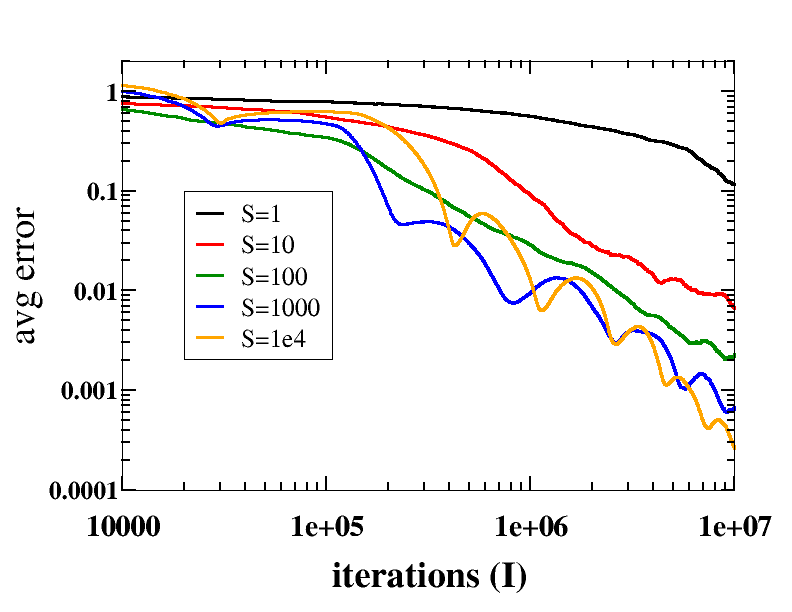
\includegraphics[width=8cm]{./figures/thirtytwo_root0_1_varyS.png}\\
(b)\\
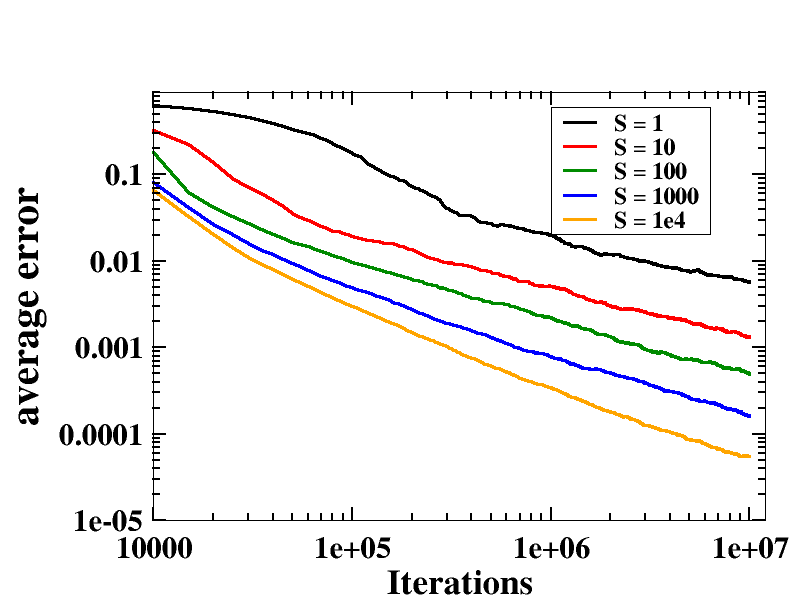
\includegraphics[width=8cm]{./figures/10X10_root1_varyS.png}
\caption{\label{thirtytwo_Stest}}
\end{figure}

Another aspect of the algorithm to consider is the dependence on the value of $N$. In Fig \ref{N_dependence} the dependence on N is shown for  the 32X32 Ising model and  10X10 ising model, simulated to $I=1e6$ and $I=1e7$ respectively, with $\mathcal{S}=100$, and averaged over 36 independant calculations. The results show that for the larger 32X32 model the dependence on $N$ is more pronounced and that the optimal value of $N$ is lower than for the smaller 10X10 model. 

\begin{figure}
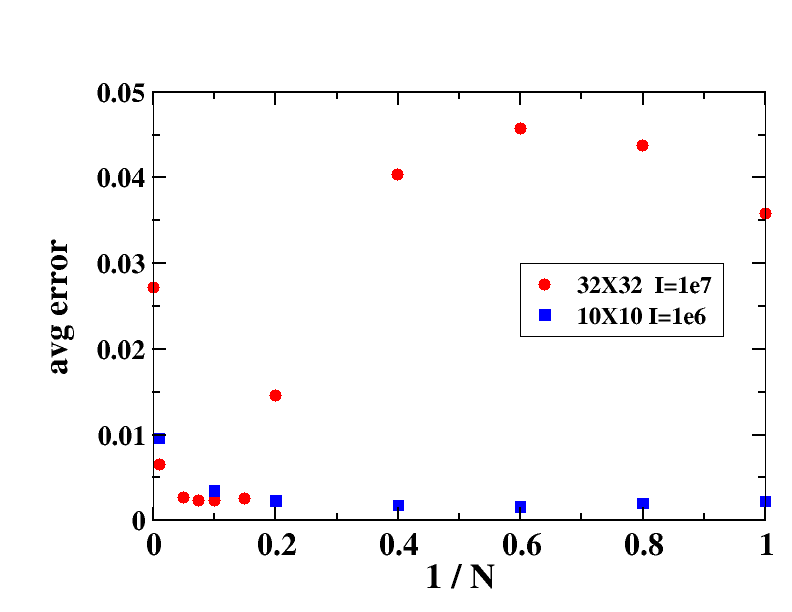
\includegraphics[width=7.5cm]{./figures/randN_3232_1010_S100.png}\\
\caption{\label{N_dependence}}
\end{figure}

The final part of this section is a compuatational test of Eq \ref{dervied_GE_GEr_relationship}. To do this first a 10$\times$10 Ising model was simulated to $2.7\%$ error to generate a $G_r(E_j)$. Then a set of 10 walkers was simulated to 1e9 iterations  with Wang and Landau importance sampling with respect to this fixed $G_r(E_j)$. In Fig \ref{GE_GEr_test} is shown plots of the ratio of the exact density of states $G(E_j)$ to the approximate relative density of states $G_r(E_j)$ and 
\begin{equation}
H(E_j) \equiv  \mathcal{H}(E_j,\{e_s\}_{\mathcal{S}\times\mathcal{I}})\frac{(\sum_j^{\Pi}\frac{G(E_j)}{G_r(E_j)})}{\mathcal{S I}}    \;.
\end{equation}
The agreement between theory and experimet(numerical) is seen to be exact within the visible precision of the plot, there as providing evidence for the valididity of Eq \ref{dervied_GE_GEr_relationship}. 

\begin{figure}
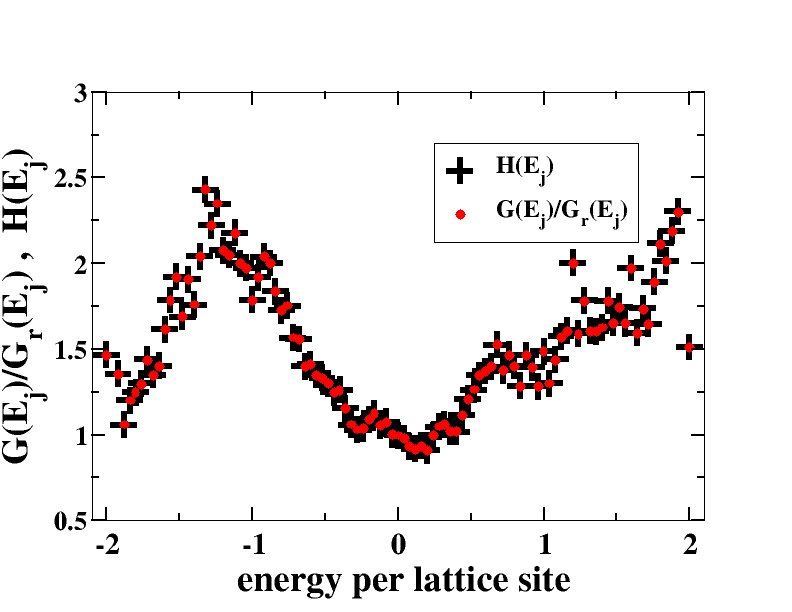
\includegraphics[width=7.5cm]{./figures/test_GE_div_Gr.png}
\caption{\label{GE_GEr_test}}
\end{figure}

\section{Application to LLTO}
The purpose of developing the B$_L$ENDER algorithm was to develop and algorithm suitable for the needs of solid state density functional theory calculations of disordered lattice materials.  Due to the long run time of density functional theory calculations  the parallel nature of B$_L$ENDER allows for calculations of each energy to be done as independant job submissions to a computer cluster. The results can then be processed by a script running on the head node.  In this work the B$_L$ENDER algorithm is applied to the lithium and lanthanum sub lattice of the solid state lithium ion electrolyte  Li$_{0.5}$La$_{0.5}$TiO$_{3}$. The goal of this study was to both, perform a calculation with B$_L$ENDER of a real material system that is fairly well understood, and also to learn something new in the process.  Specifically the desired knowledge to be gained is a better understanding the disordering of the lithium and lanthanum sub lattice and associated lattice distoritions. 

\subsection{Background on LLTO}
LLTO is a complex material comprised of a variety of stoiciometries and phases but in this work the study is restricted to the reported tetragonal P4mmm phase of the stoiciometry Li$_{0.5}$La$_{0.5}$TiO$_{3}$\cite{LLTOreview,P4mmmstrucuture}. A unit cell of this structure is shown in Fig \ref{LLTO_unit_cell}. The lattice parameters for this unit cell were taken from the experimental results from Ibarra et al.\cite{P4mmmstrucuture}; 3.8688(4)$\AA$ for a and b axes, and 7.7463(2) for c-axis.  This unit cell is representative of an ordered form of Li$_{0.5}$La$_{0.5}$TiO$_{3}$ where the lithium and lanthunum are seperated into seperate layers on the high symettry A-sites. Where the A-site refers to the general pervoskite formula unit ABX$_3$.  The structure in Fig \ref{LLTO_unit_cell} is actually strucutrally unstable and the energy can be lowered by lattice disortions which manifests as tilts in the titaninum oxygen octehedra and the lithium and lanthum distoriting off of the high symettry A-sites. The instablity of the structure in Fig \ref{LLTO_unit_cell} is evidenced by the imaginary phonon modes calculated by Moriwake et al. \cite{imaginary_phonons}.  The physics of interest in this study is to understand the disordering of lithium and lanthanum between layers.  It is reported for this phase that the lanthanum are mostly mixed between layers when the samples are slow cooled during synthesis and if quenched from high temperature the lanthanum ordering is reported to be completely mixed between layers \cite{P4mmmstrucuture}. Apart from the mixing of lithium and lanthum between layers there is also configurational complexity associated with octahedral tilting. In this work the B$_L$ENDER algorithm is used to evaluate the density of configuration states associated with local minium corresponding to both the litihium and lanthanum ordering and lattice distortions.  This lattice disortions manifest as the lithium and lanthunum sitting distorting off of the high symettry A-sites that they site on as shown in Fig \ref{LLTO_unit_cell}. 
\begin{figure}
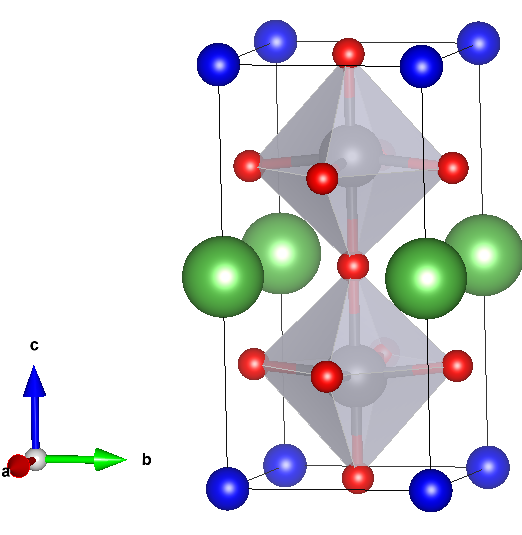
\includegraphics[width=7.5cm]{./figures/unit_cell_P4mmm_cropped.png}
\caption{10 atom unit cell of P4/mmm Li$_{0.5}$La$_{0.5}$TiO$_{3}$. Where dark blue balls are lithium, green balls are lanthanum, red balls are oxygen, and grey balls inside of octahedra are titaniu.\label{LLTO_unit_cell}}
\end{figure}
\subsection{Computational Details}
In this work a 3$\times$3$\times$1 supercell of the unit cell shown in Fig \ref{LLTO_unit_cell} was used as an approximation bulk Li$_{0.5}$La$_{0.5}$TiO$_{3}$. While not an ideal size as it is still restrictive of the possible lattice configurations and to the types of domains of octehedral tilting that can form it is the largest supercell practical for performing the configurational Monte-Carlo in this work. An important aspect of completing this study is a scheme for producing the initial and primed configurations in the iterative process of the B$_L$ENDER algorithm. The scheme used in this study was to first generate a set of lithium and lanthanum randomly placed on the high symettry A-sites where occupancy is restricted to one, then a small amount of noise was added to each lithium and lanthanum cooridnate. These confiurations were then relaxed to a local minimum which formed first set of configurations in the iterative process.  Then the primed configurations (step 2) were formed by swapping a random lithium and lanthum atom and placing them back on the high symmetry A-site along with a new amount of random noise, these configurations where then relaxed to a local minimum. The random noise off the A-site served to allow for searching the distorted lattice configuration space. 

The methods used in the calculation of the total energies of the lattice configurations of LLTO in this work were density functional theory using the VASP code. The PBE variant of generalized gradient approximation was used.  Wave functions were represented by a planve wave basis with a 425eV cut off and self consistent cycles were converged with a energy difference of 1e-5 eV. The k-point mesh was 1X1X2 shifted by 0.5 0.5 0.5 for the 3X3X1 supercells of the LiTiO6 unit cell. The calculations were performed at the experimental lattice paramaters 3.8688$\AA$ for a and b axes, and 7.7463 for c-axis. The paramaters for the B$_L$ENDER algorithm were $\mathcal{S}=10$ and $N=1$. The bin width used for determining $G_r(E_j)$ was choosen to 0.01eV. This value in bin width is approximately the same as relative errors in the calculations arising from the numerical details of the specified convergence paramaters. The value of omega was estimated as 10 times the combinatoric number of configurations of the lithium and lanthanum ordering onto the A-site  given as, 
\begin{equation}
\Omega \approx 10\frac{18!}{9!9!} \;.
\end{equation}
While an exact value of $\Omega$ is not needed for the algorithm to converge experience suggests that being close as possible is computationally beneficial. Estimating that $\Omega$ is greater than the combinatoric calculation of the lithium and lanthanum in the A-site cages comes from the possibility of multiple distinct lattice distoritions for each type of A-site cage configuration. 
\subsection{Results}
  Using the paramters and configurational enumeration scheme specified above a simulation was performed to 800 iterations for  the 3$\times$3$\times$1,  90 atom supercell. After 150 iterations the algorithm was restricted to look the in the energy range less than 1.25eV higher than the lowest energy found at that time. This was to improve compuatational efficiency by preventing the walkers from exploring an unnecessarily high energy range. While 800 iterations is likely not ideally converged, some indication of convergence can be understood by comparing the results at 400 iterations to those at 800 iterations. It is expected that the qualititave aspects of the results are well accounted for despite the limited number of iterations. 
  
  The main focus of the results is the nature of the lithium and lanthanum sublattice ordering. To accomplish this the order parameter of interest is that of the occupancy of lanthanum in the lanthanum rich layer along the c-axis.  In the work by Ibarra et al. \cite{P4mmmstrucuture} they refer to this order paramater as $La1^c$, the same convention will be used in this work. In this work the order parameter of the lanthanum rich layer along the equivalent a and b axes denoted as $La1^{a,b}$ is also studied. This is of interest becuase the system is neary cubic it is expected that the layering along the a and b axis should have similar energetics to that along the c-axis. These two order paramters, $La1^c$ and $La1^{a,b}$, are defined as the number of lanthanum in the lanthanum rich layer divived by the total number that could occupy the layer. As an example the unit cell in Fig \ref{LLTO_unit_cell} woud have $La1^c=1$ and $La1^{a,b}=0.5$  It is important to note in this work the 3$\times$3$\times$1 supercell restricts the configurations along the a and b axis from having altenerate layering of lithium and lanthanum rich layers. Ideally the calculations would be done with at least a 4$\times$4$\times$1 supercell but the computational effort is beyond the scope of this work. The results later will have to be interpreted taking this systematic supercell error into account.  
  
To calculate the ensemble average of these order paramaters first arithmetic averages of the order parameter at each energy level $E_j$ are calculated from the primed configurations ($\{\Sigma_s ^{'}\}$) that occurred during the simulation. The arithmetic average of an general order parameter $O$ over all configurations with energy $E_j$ is denoted by $< O >_j$. Then with these the ensemble average is computed as, 
  \begin{equation}
  \langle O \rangle  =  \sum_j^{\Pi}< O >_j G_r(E_j) \frac{e^{-\frac{E_j}{k_BT}}}{Z} \;.
  \end{equation}
It is noted that normalization of the relative density of states to the appropriate number of configurations is not necessary for that calculation of this order parameter. If wanting to compare free energies($-k_BT\ln(Z)$) between phases it would be necessary to normalize the density of states properly to obtain an accurate calculation of the free energy. 

\begin{acknowledgments}
This work was supported by the Center for Electrical Energy Storage: Tailored Interfaces, an Energy Frontier Research Center funded 
by the US Department of Energy, Office of Science, Office of Basic Energy Sciences at Argonne National Laboratory under Contract DE-AC02-06CH11357.
I would like to thank the Laboratory Computing Resource Center (LCRC) faculty of Argonne National Lab for their support and maintenance of the computing resources that made this project possible. 
\end{acknowledgments}
%\newcommand{\bibdir}{./}
\bibliography{Bib}
\bibliographystyle{unsrt}
\end{document}
